\documentclass{article}

%文章相关
\usepackage[UTF8, heading = false, scheme = plain]{ctex}    %解决中文字体,不改变排版
\usepackage{geometry}                                       %调整页边距等
\usepackage{indentfirst}                                    %首行缩进
\usepackage[dvipsnames,svgnames]{xcolor}                    %颜色包:\color{}
\usepackage{enumitem}                                       %控制item的前置符号
\usepackage{adjustbox}                                      %控制文字大小和添加底纹


%图片宏包
\usepackage{graphicx}                                       %插入图片:\includegraphics{myimage.png}
\usepackage{float}
\usepackage{caption}
\usepackage{subcaption}

%数学相关
\usepackage{amsmath,amsthm}                                 %amsmath包应该在前
\usepackage{extarrows}                                      %使用长等号A \xlongequal{\quad\quad}B
\usepackage{cases}                                          %\begin{numcases}可以为方程编号
\usepackage{amssymb}                                        %\checkmark 打勾

%实用的内容说明包
\usepackage{hyperref}                                       %超链接插入包:\href{url}{name}
\usepackage{multirow}                                       %插入表格用到的宏包:\begin{tabular}{|c|c|},&分列,\\分行,\hline插入横线(第二个参数是列数)
\usepackage{listings}                                       %插入代码等:\begin{lstlisting}[breaklines=true,backgroundcolor=\color{lightgray},title=]
\usepackage{verbatim}                                       %使用 comment 环境进行注释


%物理包
\usepackage{physics}
\usepackage{xparse}                                         %physics需求的包
\usepackage{mhchem}                                         %输入原子核的表式\ce{^238_92U}

% \eval{}        根据括号内容的大小在右边添加合适的竖线A|          |         \dv[n]{f}{x}          n阶微分算符 derivative
% \abs{}         添加绝对值|A|                                |         \pdv[n]{f}{x}         n阶偏微分算符 partialderivative
% \norm{}        模||A||                                     |          \bra \ket \braket    左、右、内积
% \comm{}{}      对易子[A,B]                                  |          \op{}{}              外积(密度算符) outerproduct
% \anticomm{}{}  反对易子{A,B}                                |          \ev{<力学量>}{<态>}    期望 expectationvalue
% \vb{}          向量加粗字体                                  |          \mel{}{}{}           矩阵元 matrixelement
% \va{}          向量                                        |          \mqty                 生成矩阵,可跟{} () [] || &分列 \\分行 第一个表示外面无框
% \vu{}          单位向量                                     |         \qty                  合适大小的{}、()等,例如 \qty(x)
% \vdot          点乘                                        |
% \cross         叉乘                                        |
% \grad          梯度 gradient                               |
% \div           散度 divergenc                              |
% \curl          旋度                                        |
% \laplacian     拉普拉斯算符                                 |

%文本底纹实现
\usepackage{lipsum}                                         %该宏包是通过 \lipsum 命令生成一段本文,正式使用时不需要引用该宏包
\usepackage[strict]{changepage}                             %提供一个 adjustwidth 环境
\usepackage{framed}                                         %实现方框效果
%\usepackage{newtxtext}                                     %在macos会报错的一个包注释掉不影响使用
\usepackage{tcolorbox}                                      %文本底纹包,放在xcolor包后
                               
% environment derived from framed.sty: see leftbar environment definition
\definecolor{formalshade}{rgb}{0.95,0.95,1}% 文本框颜色
% ------------------******-------------------
% 注意行末需要把空格注释掉,不然画出来的方框会有空白竖线
\newenvironment{formal}{%
\def\FrameCommand{%
\hspace{-1em}%                                              %框的整体缩进
{\color{Green}\vrule width 0.3em}%                          %竖线颜色以及宽度
\colorbox{greenshade}%                                      %底纹颜色
}%
\MakeFramed{\advance\hsize-\width\FrameRestore}%
\noindent\hspace{-2em}%                                     %禁止第一段文本缩进
\begin{adjustwidth}{}{2em}%                                 %控制右边距        
\vspace{1.5em}%                                             %控制上边距
}
{%
\vspace{1.5em}\end{adjustwidth}\endMakeFramed%              %控制底边距
}%

\definecolor{greenshade}{rgb}{0.90,0.99,0.91}               %绿色文本框,竖线颜色设为 Green
\definecolor{redshade}{rgb}{1.00,0.90,0.90}                 %红色文本框,竖线颜色设为 LightCoral
\definecolor{brownshade}{rgb}{0.99,0.97,0.93}               %莫兰迪棕色,竖线颜色设为 BurlyWood


%使用Mathematica进行计算
%\usepackage{latexalpha2}
%/usr/local/texlive/texmf-local/tex/latex/local/latexalpha2
%直接使用wolfram代码
% \wolfram[<format>]{<code>}    \wolframgraphics[<format>]{<code>}{<filename>} 
%具体使用方法查看 latexalpha2.pdf


%预设
\geometry{a4paper,left=5em,right=5em,bottom=5em,top=5em}    %设置为a4paper最好,点击pacakge geometry 查看文档
\setlength{\parindent}{2em}                                 %2em(注意不支持rem)代表每一段的首行缩进两个字符,某一行不缩进时使用 \noindent

\hypersetup{hidelinks,colorlinks=true,
linkcolor=black,urlcolor=blue}                              %对hyperref 包进行预设

\newenvironment{slt}{\proof[\indent \bf 解 ]}{
\renewcommand{\qedsymbol}{}\endproof}                       %提供解环境
\newtheorem{thm}{定理}[section]                              %定义一个新的环境 thm, 命名为定理,以 节 开始编号
\newtheorem*{thm*}{定理}                                     %定义一个新的环境 thm, 命名为定理,无编号
\newtheorem{lemma}{引理}[section]                            %定义新环境 lemma,命名为引理,以 节 开始编号
\newtheorem*{lemma*}{引理}                                   %定义新环境 lemma,命名为引理,无编号
\newtheorem{corollary}{推论}                                 %定义新环境 corollary,命名为推理,有编号
\newtheorem*{corollary*}{推论}                               %定义新环境 corollary*,命名为推理,无编号
\renewcommand{\proofname}{ \qquad \bf 证明}                  %更改proof为中文证明,proof环境默认存在

%一些def
\def\thmindent{\setlength{\parindent}{5em}}                  %\thmindent
\def\pfindent{\setlength{\parindent}{5.5em}}                 %\pfindent
\def\clindent{\setlength{\parindent}{4em}}                   %clindent
\def\sdr{Schr\"{o}dinger}                                    %薛定谔名字
\def\intff{\int_{-\infty}^{+\infty}}                         %积分为(-\infty,+\infty)的积分
\def\ra{\rightarrow}                                         %右键头\ra
\def\lra{\Longrightarrow}                                    %长(双)右键头\lra
\def\lla{\Longleftarrow}                                     %长(双)左键头\lla
\def\llra{\Longleftrightarrow}                               %等价箭头\llra
\def\xlra{\xlongrightarrow{\quad\quad}}                      %超长右箭头
\def\xlla{\xlongleftarrow{\quad\quad}}                       %超长左箭头
\def\xlla{\xlongleftrightarrow{\quad\quad}}                  %超长等价箭头

\def\psii#1{\psi_{#1}}                                       %常用的\psi下标
\def\psiii#1#2{\psi_{#1} (#2)}                               %常用的\psi下标和括号
\def\psiiii#1#2#3{\psi_{#1}^{#2} (#3)}                       %常用的\psi下标、上标和括号
\def\pe#1#2{E_{#1}^{(#2)}}                                   %能量修正{下标}{上标}
\def\pp#1#2{\psi_{#1}^{(#2)}}                                %波函数修正
\def\ua{a_{+}}                                               %升算符
\def\da{a_{-}}                                               %降算符

\def\nuc#1#2#3{\ce{^{#1}_{#2}{#3}}}                          %原子核的表示形式


%其他备注
\begin{comment}
        求和指标上下方添加        \sum\limits_{}^{}
        恒等于                  \equiv
        远大于                  \gg
        远小于                  \ll
        花括号                  \left\{ \right\}   (建议使用\qty)
        弧度                    37^{\circ}


\end{comment}


%作业包(需要的时候再解除注释)
%\usepackage{iidef}
%建议使用自己的slt解环境
\begin{comment}

    package iidef:
        指定学校名      \thecourseinstitute{}      
        指定课程名      \thecoursename{} 
	    指定学期        \theterm{}
        作业名         \hwname{}
        生成作业标题    \courseheader           放在document环境内 不需要再maketile
        名字           \name                   放在document环境内
        自动编号环境    \begin{enumerate}       [label = (\alph*{})] [label = \arabic*{}.]
        题号           \item                   自动编号,\item[]则不带符号
        证明           \begin{proof}           证明环境由amsthm包提供
        求解           \begin{solution}       
        方程           \begin{equation}        
        方程编号        \labe{eq:[number]}      为方程设置编号  
        引用方程        \eqref{eq:[number]}     引用方程
        行内方程        $...$
        
        多行公式        \begin{align} \begin{align*}则不会编号  
                            ... & = ... \\ 
                                & = ...
                       \begin{array}{lcl}      
                            ... & = & ... \\ 
                            ... & = & ...
        
        方程组          $$
                        \begin{cases}
                       ... & \mbox{if} x \mbox{is even} \\ 带假设
                       $$
                       
                       带编号
                       \begin{numcases}{}
                            \label{1}   \\
                            \label{2}   
                       \end{numcases}
        
        文字大小和底纹
                       \vspace{-1em}
                       \begin{adjustbox}{minipage=0.91\linewidth, bgcolor=gray!20, padding=1em}
                       \small % 将字号变小为 small
                        text
                       \end{adjustbox}
                       \vspace{-1em}

        居中            不要使用$$...$$,会对齐失效 使用$...$即可
                        \begin{center}
            
                        \end{center}

        左对齐           
                        \begin{flushleft}
            
                        \end{flushleft}

        双水平图         \begin{minipage}{0.45\textwidth}
                        \includegraphics[width=\textwidth,keepaspectratio]{./pictures/.png}
                        \end{minipage}
                        \hfill
                        \begin{minipage}{0.45\textwidth}
                            \begin{enumerate}[label = (\arabic*)]
                                \item 
                                \item 
                                \item 
                            \end{enumerate}
                        \end{minipage}

    
\end{comment}





\title{高中物理}
\author{马祥芸}


\begin{document}
\maketitle
\tableofcontents
\zihao{-4}
\newpage

\section{匀变速直线运动问题}

\subsection{中间时刻/平均速度}
中间时刻速度$v_{\frac{t}{2}}$与平均速度$\overline{v}$是同一个值
$$
    v_{\frac{t}{2}} = v_{0} + \frac{at}{2} = \frac{v_{0}}{2} +  (\frac{v_{0}}{2} + \frac{at}{2})   = \frac{v_{0}+v_{t}}{2} = \overline{v}
$$

中间位置速度

\begin{numcases}{}
    \label{1} 2 a\frac{x}{2} = v_{\frac{x}{2}}^{2} - v_{0}^{2}  \\
    \label{2} 2 a\frac{x}{2} = v_{t}^{2} - v_{\frac{x}{2}}^{2}
\end{numcases}

由方程$(1) - (2)$ 得到 $ v_{\frac{x}{2}} = \sqrt{\frac{v_{0}^{2} + v_{t}^{2}}{2}} $

\subsection{纸带加速度问题}
纸带的特点,每个计时点的时间间隔相同均为$T$,且$x_{n}$规定的是第$n$个时间间隔内的位移,并非到起点的距离

\begin{corollary*}
    相邻位移之间的差为$aT^{2}$,等时位移比例式为$x_{1}:x_{2}:x_{3} : \dots : x_{n} = 1:3:5: \dots :2n-1  $
\end{corollary*}
\begin{proof}
    \begin{align*}
        x_{n} = \frac{1}{2}a (nT)^{2} -  \frac{1}{2}a [(n-1)T]^{2} & = aT^{2} (\frac{2n-1}{2}) \\
        x_{n-1}                                                    & = aT^{2} (\frac{2n-3}{2}) \\
        x_{n} - x_{n-1}                                            & = aT^{2}
    \end{align*}
\end{proof}

\begin{corollary*}
    等位移比例式子($1m$,$2m$,$3m \dots$)    \\
    前$1m,2m,3m \dots n \, m$所用时间比为$1:\sqrt{2}:\sqrt{3}:\dots:\sqrt{n}$,若是第$i\,m$内则向前减一个就行
    \begin{proof}
        \begin{align*}
            1 & = \frac{1}{2}a t_{1}^{2} \lra t_{1} =\sqrt{\frac{2}{a}} \vdot \sqrt{1} \\
            2 & = \frac{1}{2}a t_{2}^{2} \lra t_{2} =\sqrt{\frac{2}{a}} \vdot \sqrt{2} \\
            3 & = \frac{1}{2}a t_{3}^{2} \lra t_{3} =\sqrt{\frac{2}{a}} \vdot \sqrt{3} \\
            n & = \frac{1}{2}a t_{n}^{2} \lra t_{n} =\sqrt{\frac{2}{a}} \vdot \sqrt{n} \\
        \end{align*}
    \end{proof}
\end{corollary*}

\vspace{2em}

\section{机械振动}
\subsection{简谐振动}
\begin{itemize}
    \item 定义: 具有平衡位置,回复力形如$F_{\text{回}} = -kx$(来自合外力或其分力)
    \item 振子方程: $\sin{(\omega t + \varphi)}$
    \item 同侧法: 质点振动速度方向$v_{f}$与波传播方向$u$在正弦函数线的同一侧
    \item 摆周期: $T = 2\pi \sqrt{\frac{L}{g}}$
    \item 受迫振动:在周期性外力的持续作用下而进行的振动称为\textbf{受迫振动},振动稳定后齐\textbf{频率}等于外力驱动频率
    \item 等效绳长与等效加速度问题:
          \begin{itemize}
              \item 等效绳长: 确定为简谐振动,通过几何关系确定摆心
              \item 等效加速度: 主要区别电梯摆和电场摆,前者需要变换参考系(非惯性力)
          \end{itemize}
    \item  造成波的多解性的三大原因:
          \begin{itemize}
              \item \textbf{波的周期性:}\hspace{1em}
                    $\begin{cases}
                            \text{时间周期性:时间间隔}\triangle t \text{与周期} T \text{的关系不明确} \\
                            \text{空间周期性:波传播距离}\triangle x \text{与波长} \lambda \text{的关系不明确}
                        \end{cases}$

              \item \textbf{波的双向性:}\hspace{1em}
                    $\begin{cases}
                            \text{传播方向双向性:波的传播方向不确定} \\
                            \text{振动方向双向性:质点振动方向不确定}
                        \end{cases}$

              \item \textbf{波形隐含性:}\hspace{1em}
                    $\begin{cases}
                            \text{在波动问题中,有时只给出几个特殊点} \\
                            \text{(大多是两个特殊的点)的运动状态,其余信息均处于隐含状态}
                        \end{cases}$
          \end{itemize}
\end{itemize}

\vspace{2em}


\subsection{数学准备}
\begin{formal}
    \begin{itemize}
        \item 展开
              $$ \sin{(\theta \pm \beta)} = \sin{\theta}\cos{\theta} \pm \cos{\theta}\sin{\theta} $$
              $$ \cos{(\theta \pm \beta)} = \cos{\theta}\cos{\theta} \mp \sin{\theta}\sin{\theta} $$
              $$ \tan{(\theta \pm \beta)} = \dfrac{\tan{\theta} \pm \tan{\beta}}{1 \mp \tan{\theta}\tan{\beta}}$$

        \item 余补关系
              $$ \sin{(\pi - \theta)} = \sin{\theta} \quad \cos{(\pi - \theta)} = - \cos{\theta} \quad \tan{(\pi - \theta)} = -\tan{\theta}$$

              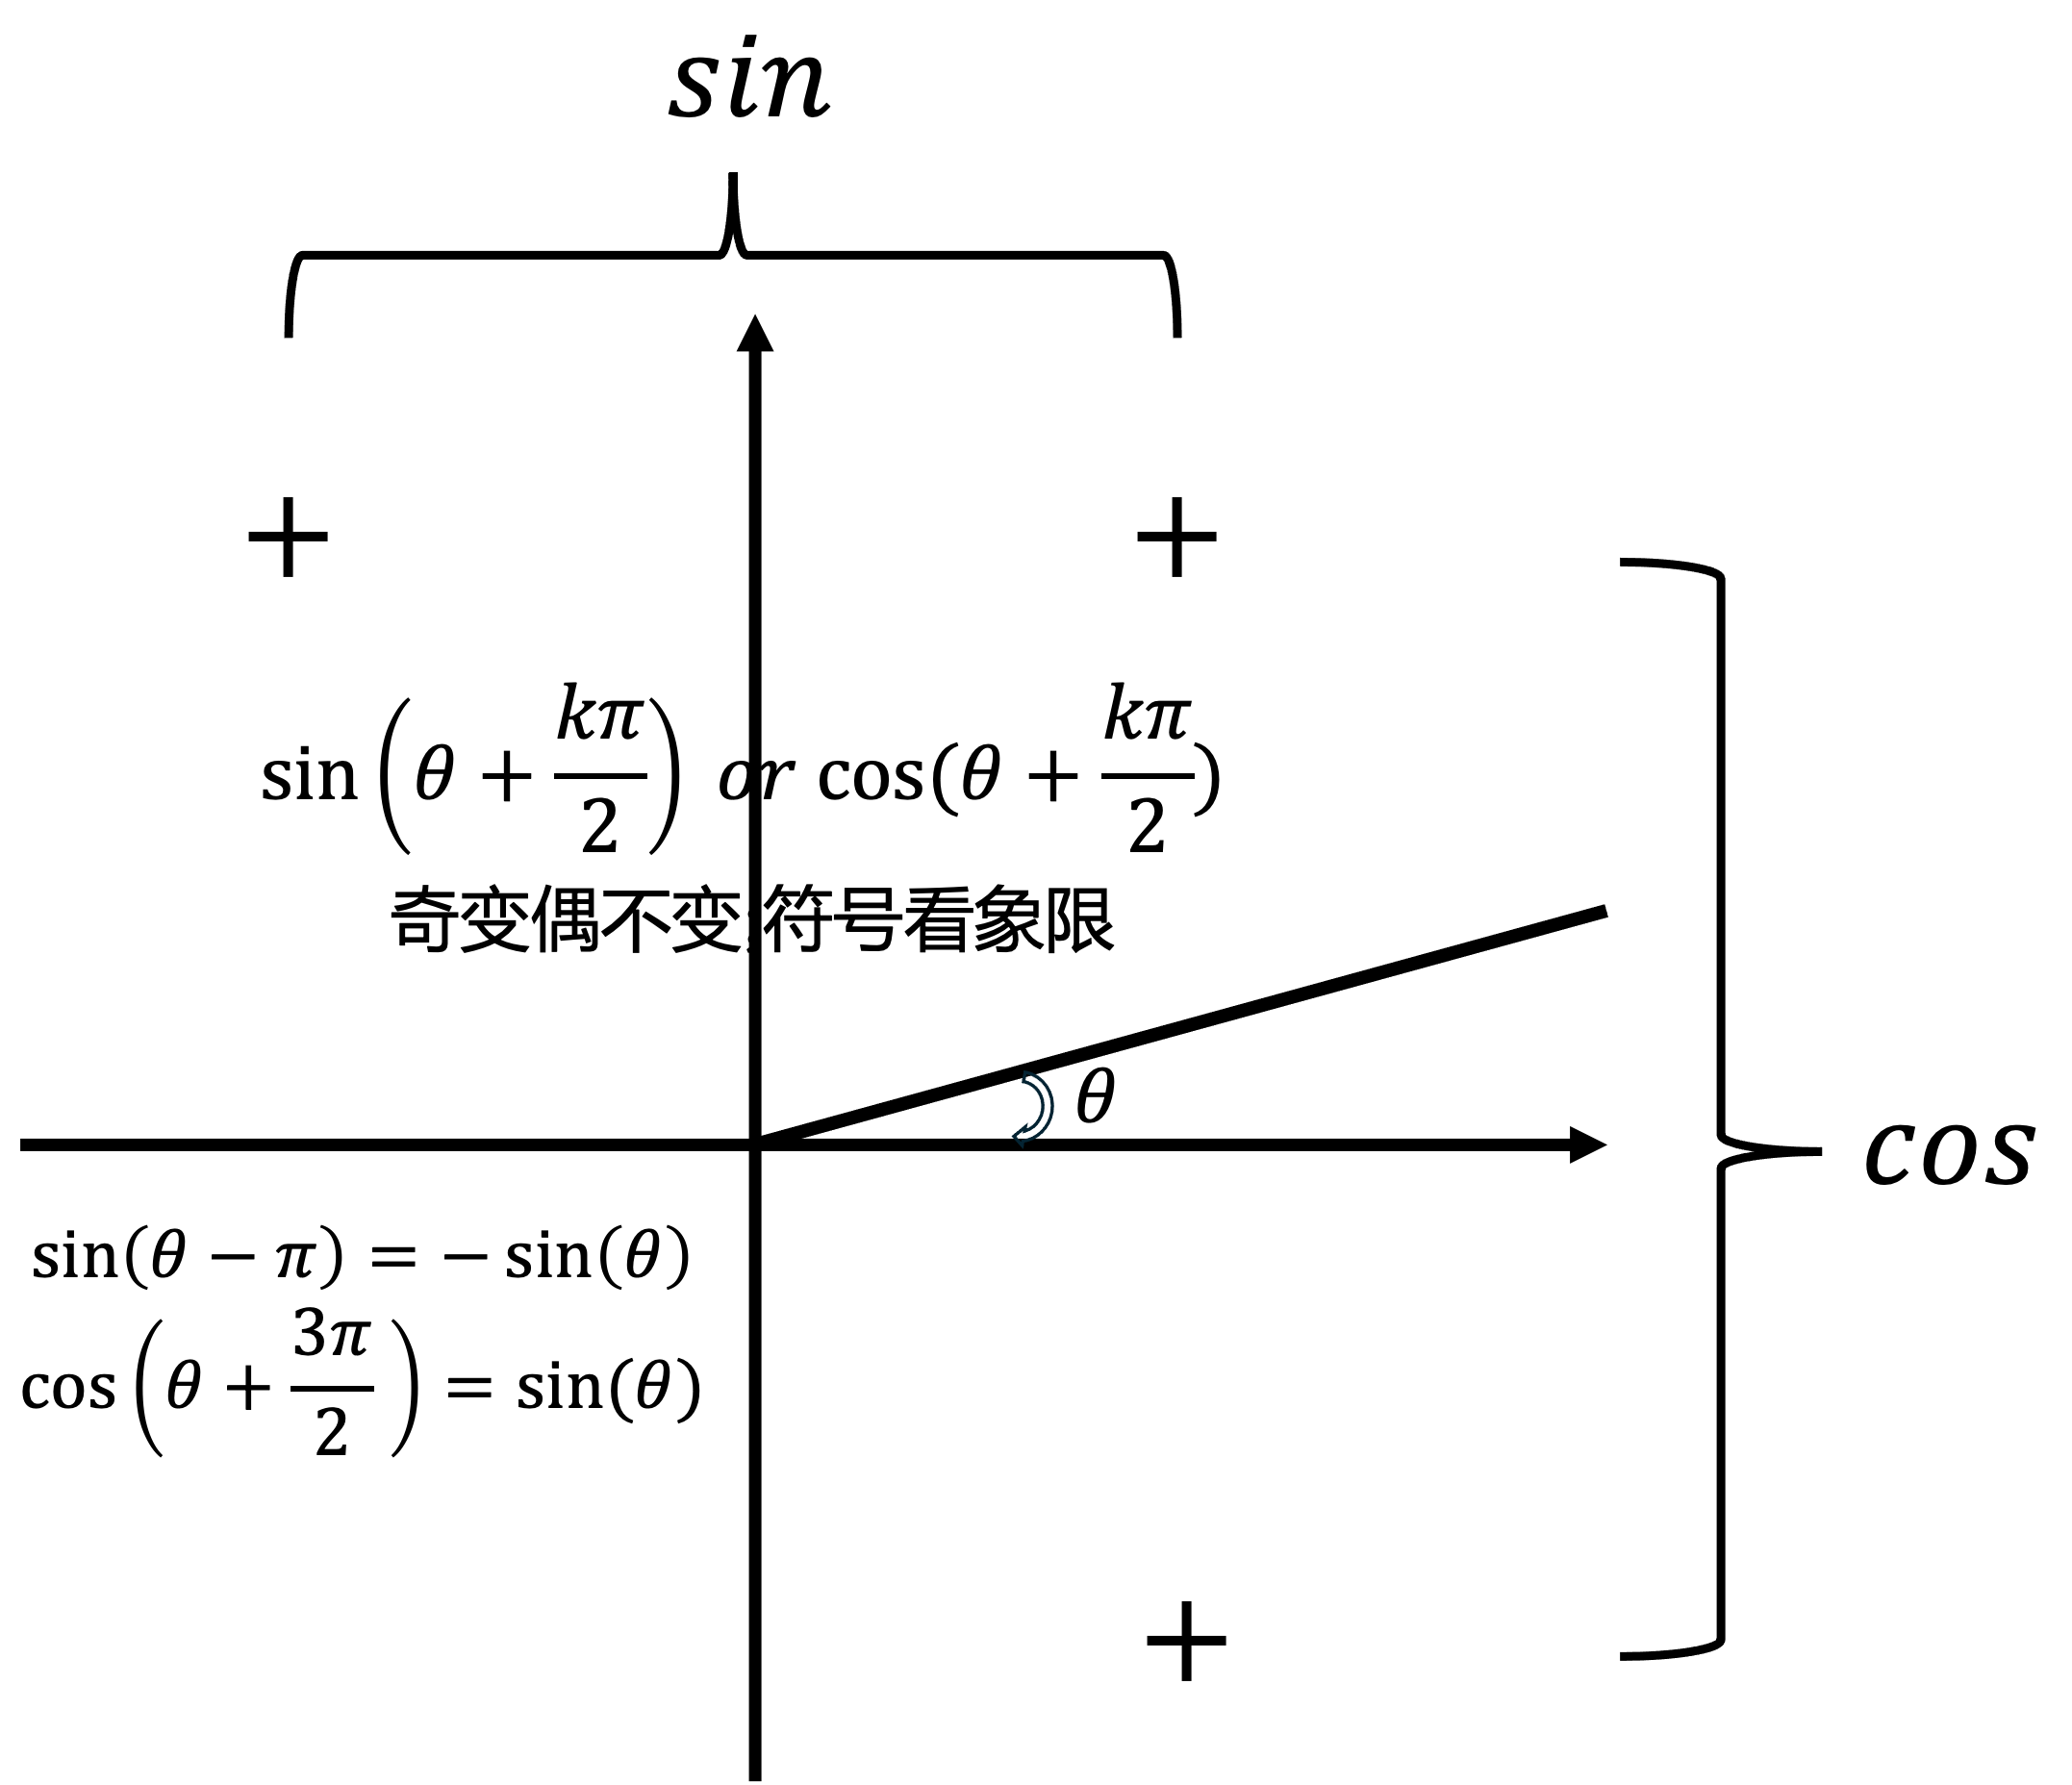
\includegraphics[width = 20em]{./pictures/1.png}

        \item 和关系
              $$ \sin^{2}{\theta}+\cos^{2}{\theta} = 1$$

        \item 正弦定理
              $$ \dfrac{a}{\sin{\alpha}} = \dfrac{b}{\sin{\beta}} = \dfrac{c}{\sin{\gamma}}   $$

        \item 余弦定理
              $$ \cos{\gamma} = \dfrac{a^{2}+b^{2} - c^{2}}{2ab} $$

        \item 二倍角
              $$ \sin{2\theta} = 2\sin{\theta}\cos{\theta} \quad \cos{2\theta} = \cos^{2}{\theta} - \sin^{2}{\theta} \quad \tan{2\theta} = \dfrac{2\tan{\theta}}{1-\tan^{2}{\theta}}$$

        \item 降次
              $$ \sin^{2}{\theta} = \dfrac{1 - \cos{2\theta}}{2} \quad \cos^{2}{\theta} = \dfrac{1 + \cos{2\theta}}{2} \quad \tan^{2}{\theta} = \dfrac{1-\cos{2\theta}}{1+\cos{2\theta}}$$
    \end{itemize}
\end{formal}

\vspace{2em}

\vspace{2em}

\section{光学}
\subsection{折射率}

\begin{itemize}
    \item 定义式:
          $$
              n = \dfrac{\sin{\text{大角}}}{\sin{\text{小角}}}
          $$
    \item 决定式:
          $$
              n = \dfrac{c}{v}
          $$
    \item 全反射:
          \begin{align*}
               & \text{光密介质} \, \ra \, \text{光疏介质} \quad \sin{\text{大角}} = 1 \,(\text{大角} = \frac{\pi}{2}) \\
               & \text{临界角} \quad \sin{C} = \frac{1}{\sin{\text{小角}}}
          \end{align*}
    \item 视深与视高:
          \begin{itemize}
              \item[] $H$为物点距离界面的高度;\,$h$为像点距离界面的高度
              \item 视深: \quad
                    从介质外看向介质内 \quad $h = \frac{1}{n} H$
              \item 视高: \quad
                    从介质内看向介质外 \quad $ h = n H $
          \end{itemize}
    \item 实验误差分析:
          \begin{itemize}
              \item 非平行玻璃砖 $\quad n_{\text{测}} = n_{\text{真}}$
              \item 整体平移  $\quad d_{\text{测}} = d_{\text{玻}} \quad n_{\text{测}} = n_{\text{真}}$
              \item 其他情况  $\quad n_{\text{测}} \text{和} n_{\text{真}} \text{的大小关系} \,\text{与}\, d_{\text{测}} \text{和} d_{\text{玻}}\text{的大小关系相反}$
          \end{itemize}
\end{itemize}

\vspace{2em}

\subsection{干涉实验}
\begin{itemize}
    \item[] 薄膜干涉: $\delta = 2d$
        \begin{itemize}
            \item[] 明暗条纹位置由波长和此处厚度共同决定
            \item[] 相邻明(暗)条纹对应的薄膜厚度差为$\frac{\lambda}{2} \quad \lambda$应为光在介质中传播时的波长
        \end{itemize}
    \item[] 劈尖干涉: 样板下表面和被检查平面的上表面的反射光发生干涉

        \hspace{5em}(标准板的厚度太厚大于相干长度)

        \begin{itemize}
            \item[] 验平问题:
                \begin{itemize}
                    \item[] 若待测板平整,干涉条纹等距
                    \item[] 若条纹\textbf{偏头},则条纹提前出现,此处光程差偏大,因此待测样板此处凹
                    \item[] 若条纹\textbf{偏尾},则条纹延后,此处光程差偏小,因此待测样板此处凸
                \end{itemize}
            \item[] 条纹间距问题:
                \begin{itemize}
                    \item[] 薄片(支撑两个板)的移动改变$\theta$角 $\quad \triangle l = \dfrac{\triangle d}{\tan{\theta}} \quad
                            \triangle d = f(\lambda) = \dfrac{\lambda}{2}$
                \end{itemize}
            \item[] 增反膜;增透膜: 入射光能量 = 折射光能量 + 反射光能量

                \hspace{4em}(注:光疏到光密反射光产生半波损失,$n_{\text{膜}}$介于空气和另一介质之间)

                \hspace{4em}增透膜:反射光相消$2d = \frac{\lambda}{2} (2n+1)$

                \hspace{4em}增反膜:反射光相长$2d = \frac{\lambda}{2} (2n) $
        \end{itemize}

    \item[] 双缝干涉: $\triangle d = \lambda \dfrac{L}{d} \,$ (条纹间距$\triangle d $,双缝间距$d$,缝板距离$L$)
\end{itemize}

\vspace{2em}

\subsection{总结}
\begin{formal}
    符号说明

    \begin{tabular}{|c|c|c|c|c|c|c|c|c|c|}
        \hline
        频率  & 折射率 & 速度  & 临界角 & 波长        & 动量  & 干涉            & 能量            & 逸出功     & 逃逸光子动能  \\
        \hline
        $f$ & $n$ & $v$ & $C$ & $\lambda$ & $p$ & $\triangle x$ & $\varepsilon$ & $w_{0}$ & $E_{k}$ \\
        \hline
    \end{tabular}

    \vspace*{2em}

    \begin{itemize}
        \item 同一介质中不同频率的光

              \vspace*{1em}
              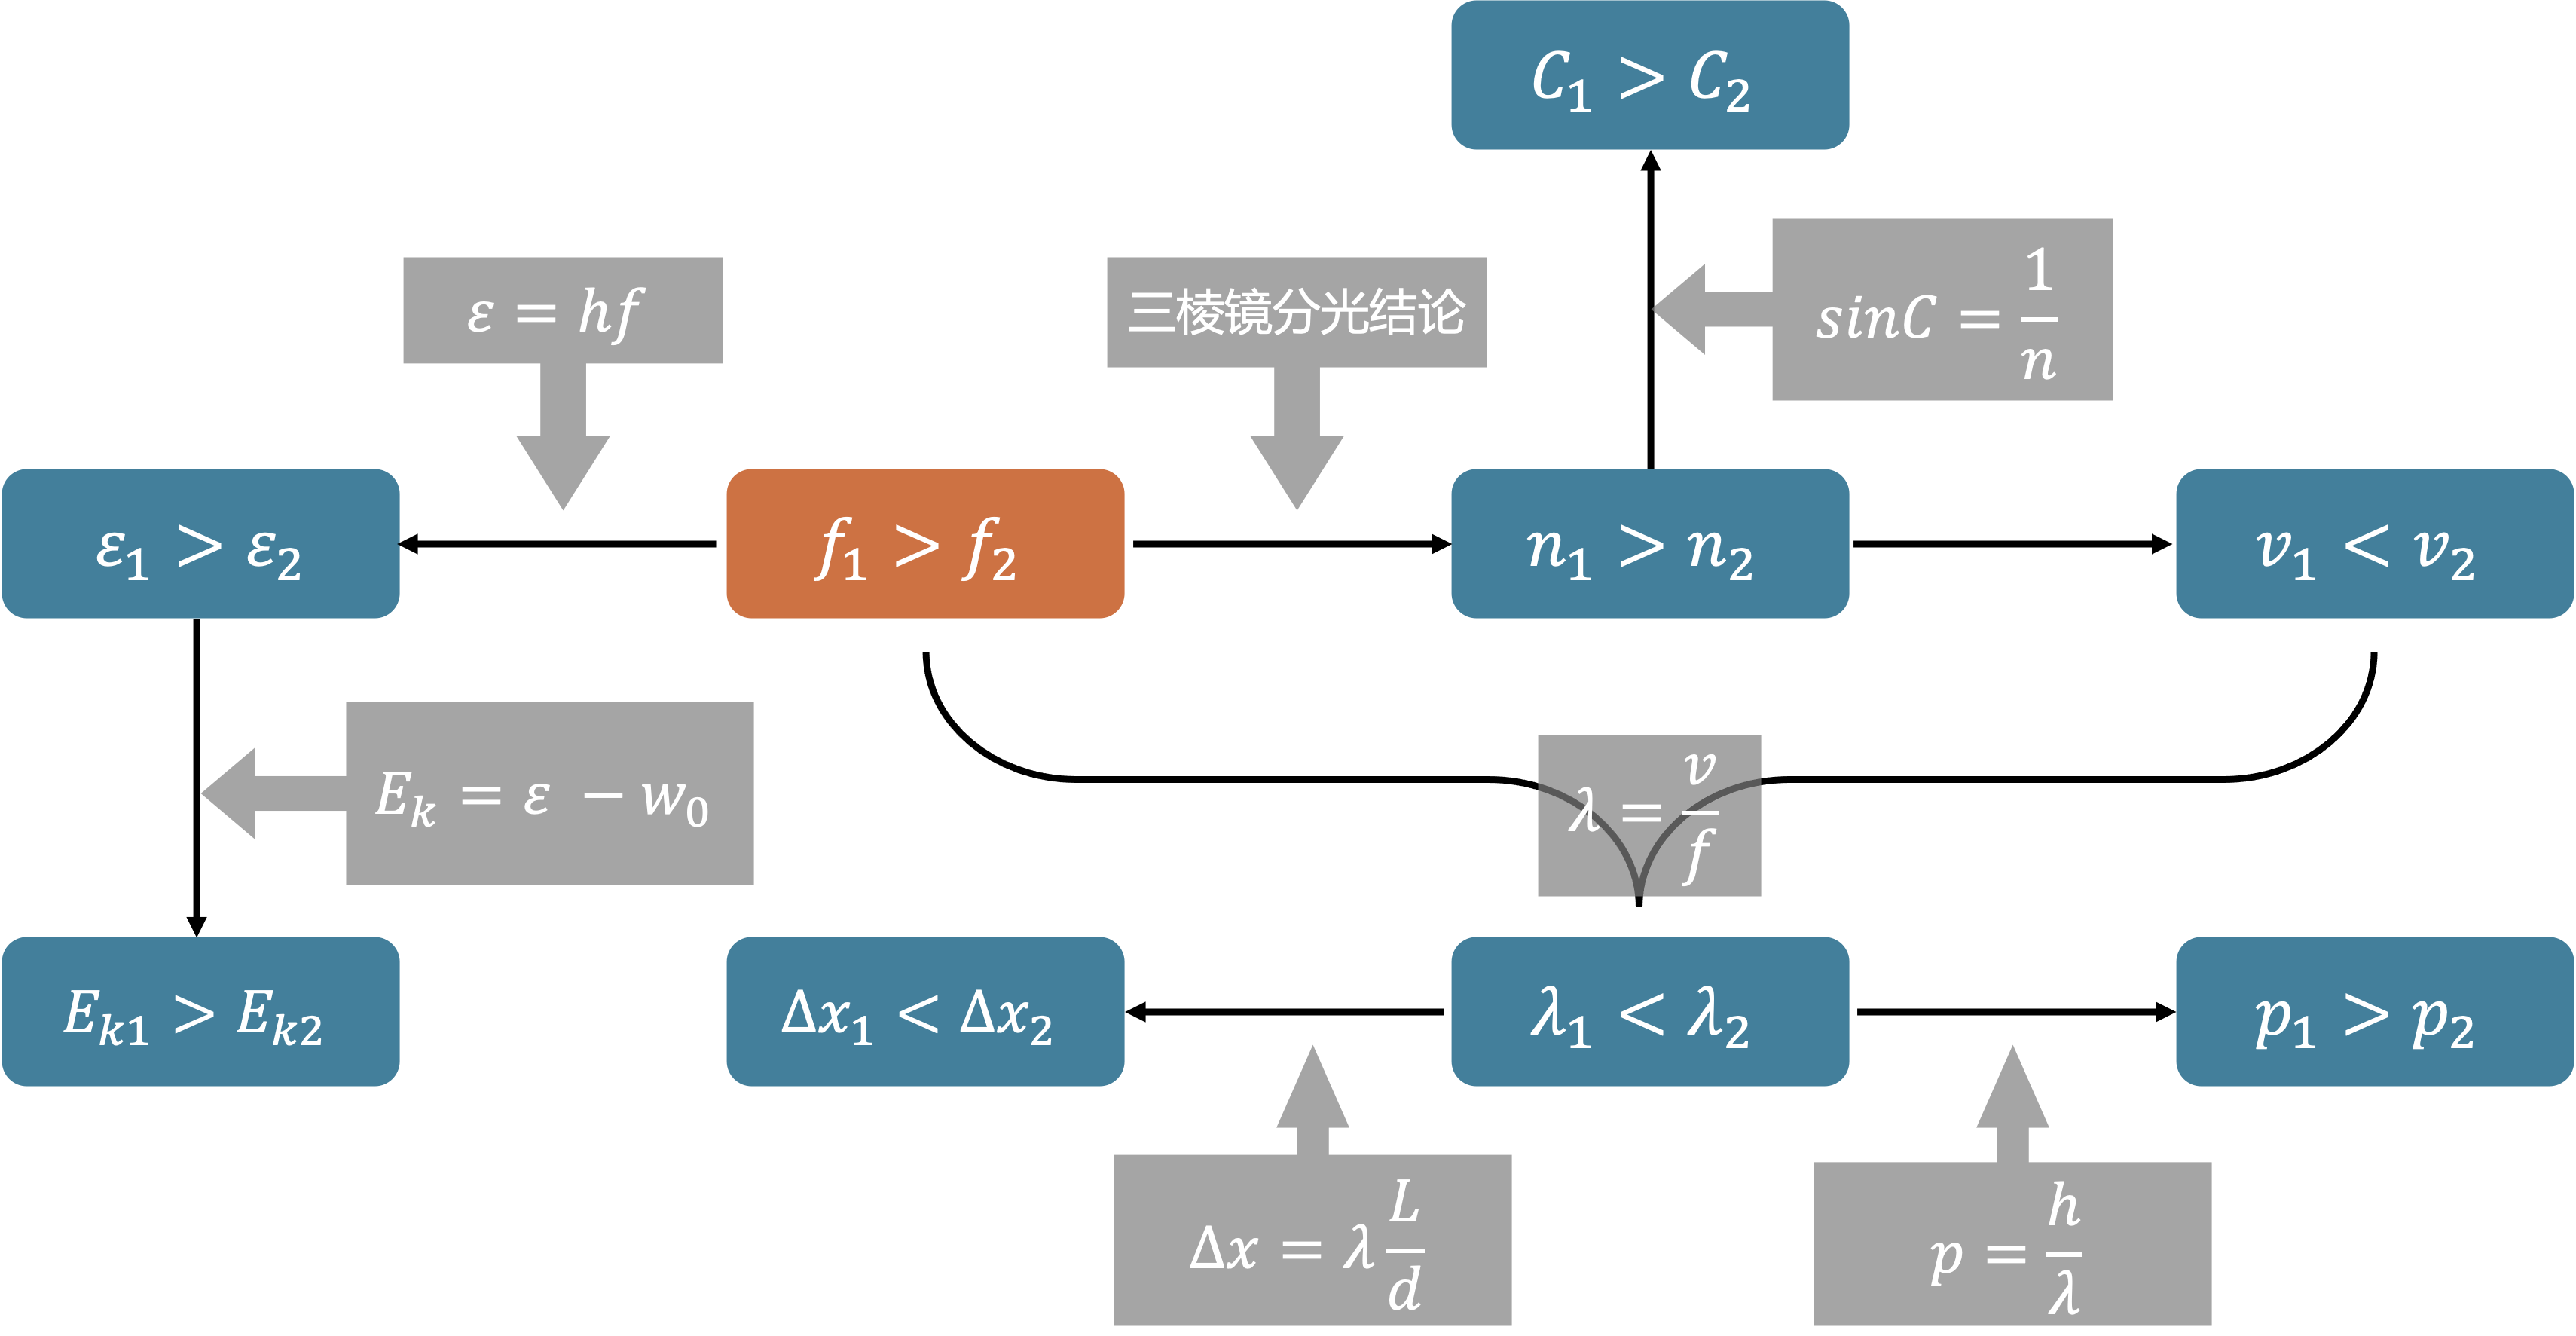
\includegraphics[width=35em,keepaspectratio]{./pictures/2.png}

              \vspace*{2em}

        \item 同一频率的光在不同介质(下标表示不同介质中)中

              \vspace*{1em}
              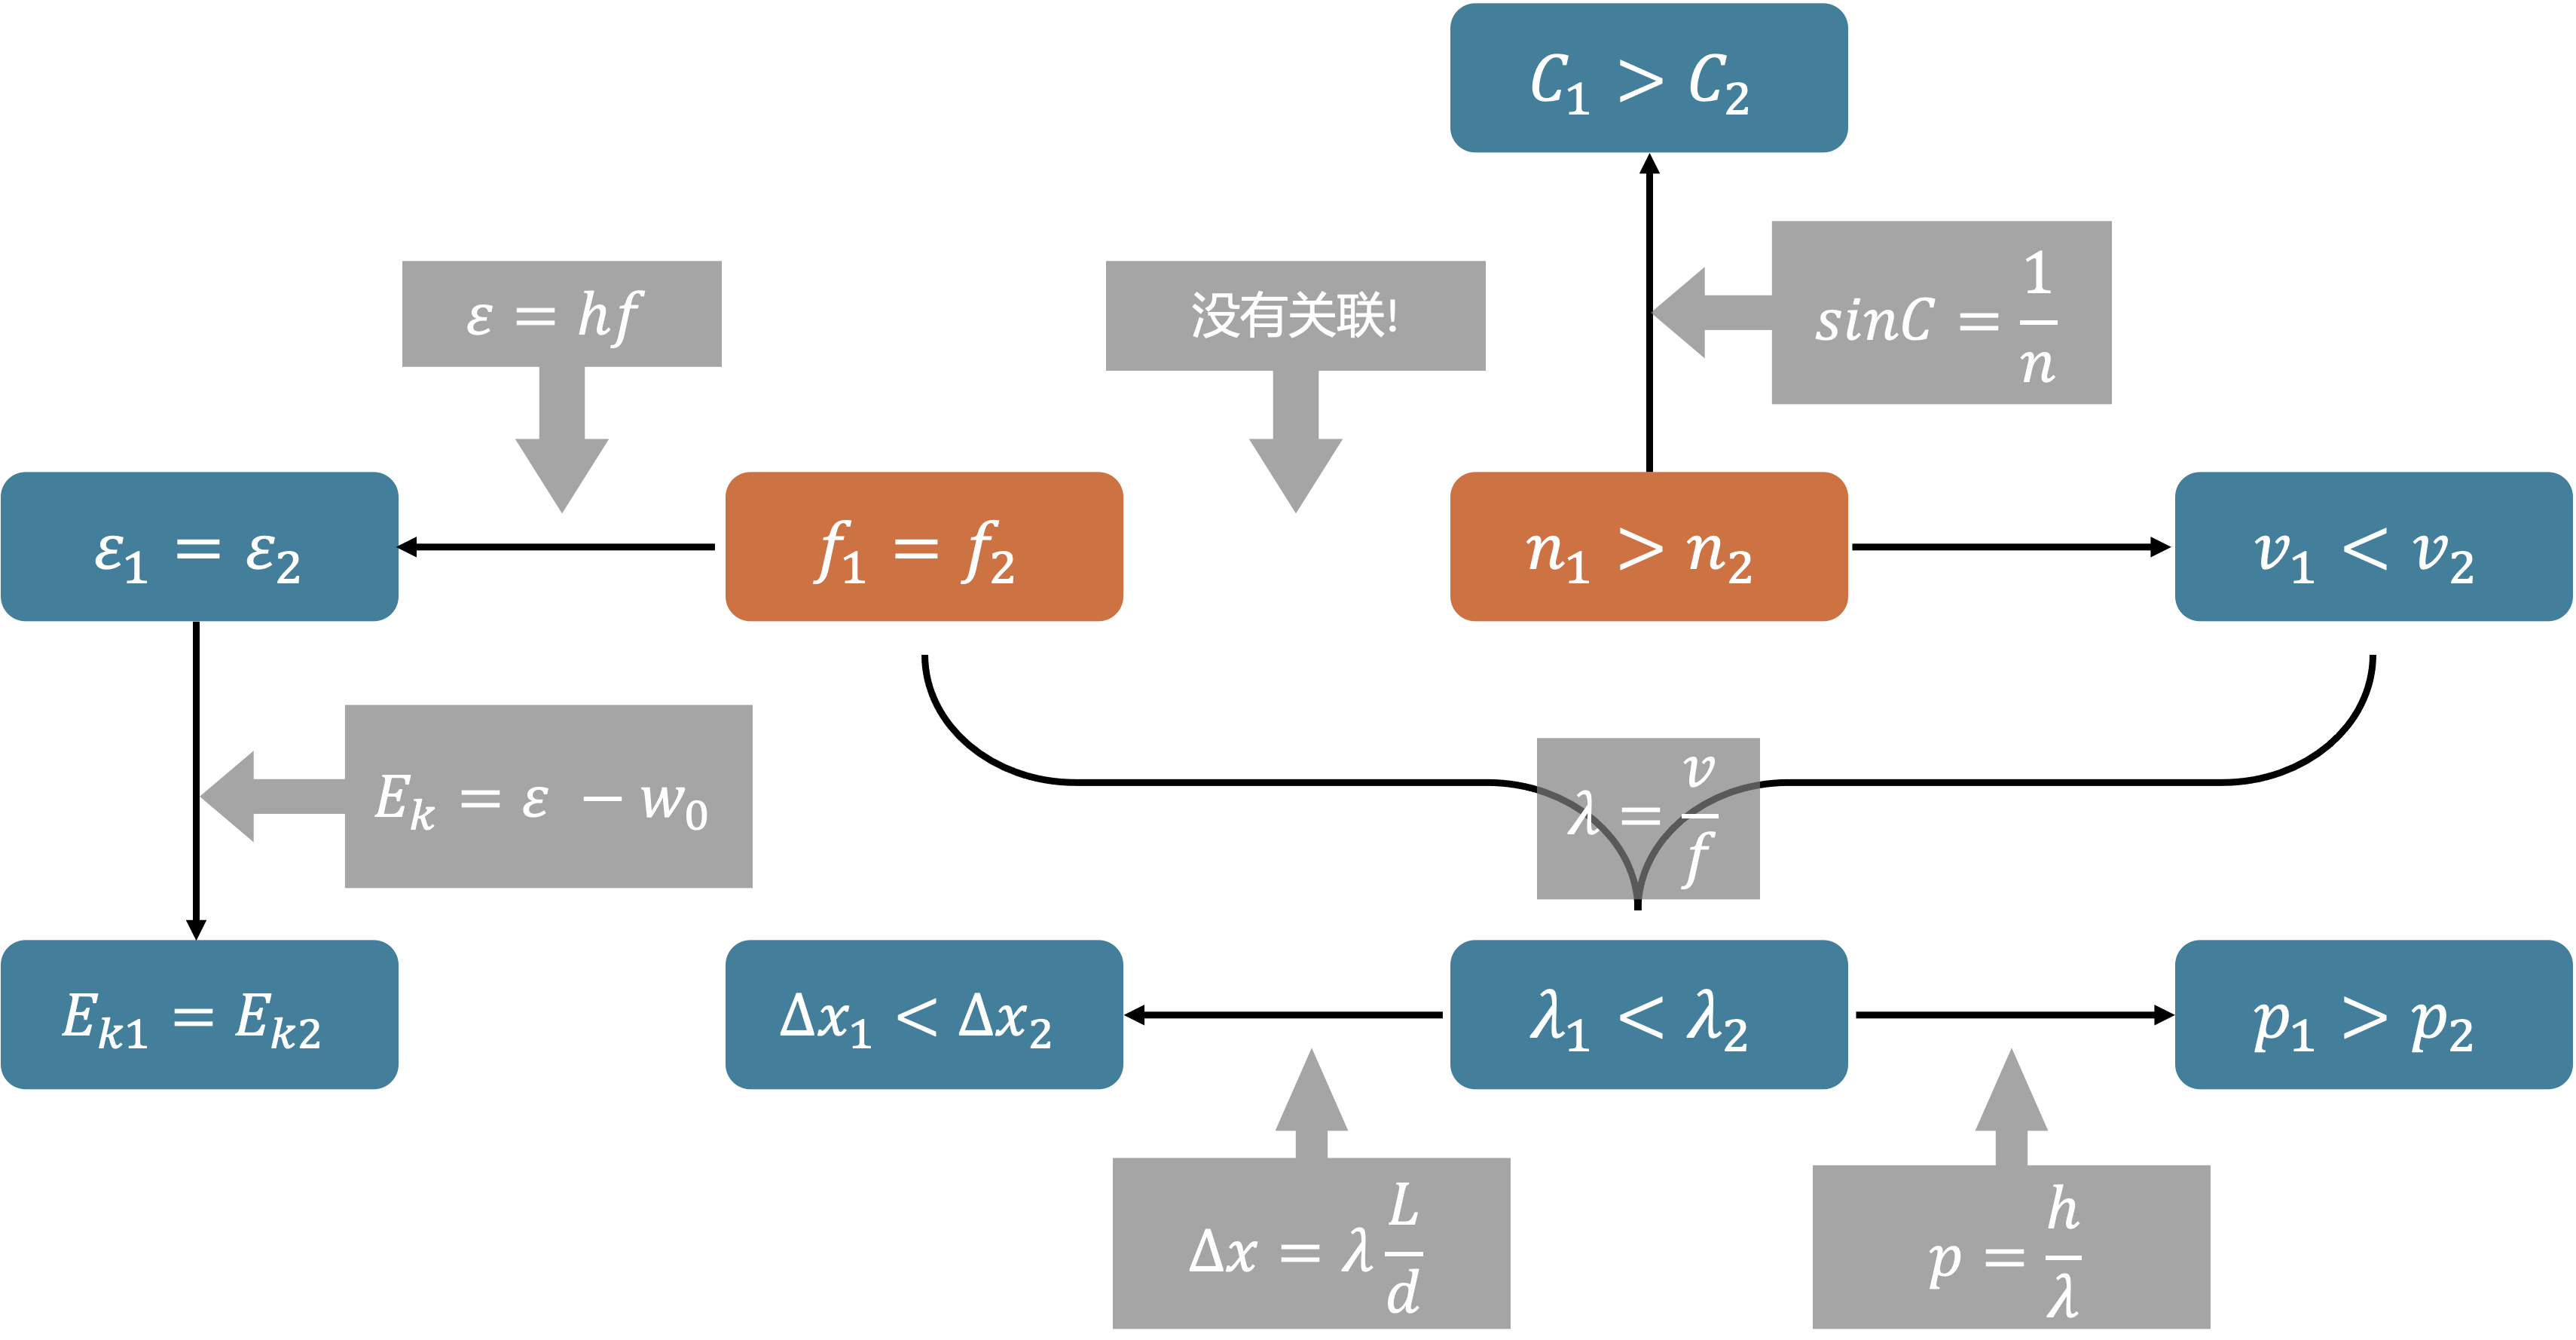
\includegraphics[width=35em,keepaspectratio]{./pictures/3.png}
    \end{itemize}
\end{formal}

\vspace{2em}

\section{热学}
\subsection{黑体辐射}

\subsubsection{物理大厦上的"两朵乌云"}
\begin{itemize}
    \item 迈克尔逊-莫雷实验: 测量假想介质\,\textbf{以太}\,(绝对参考系)$\lra$否定以太得到狭义相对论

          \vspace{1em}

          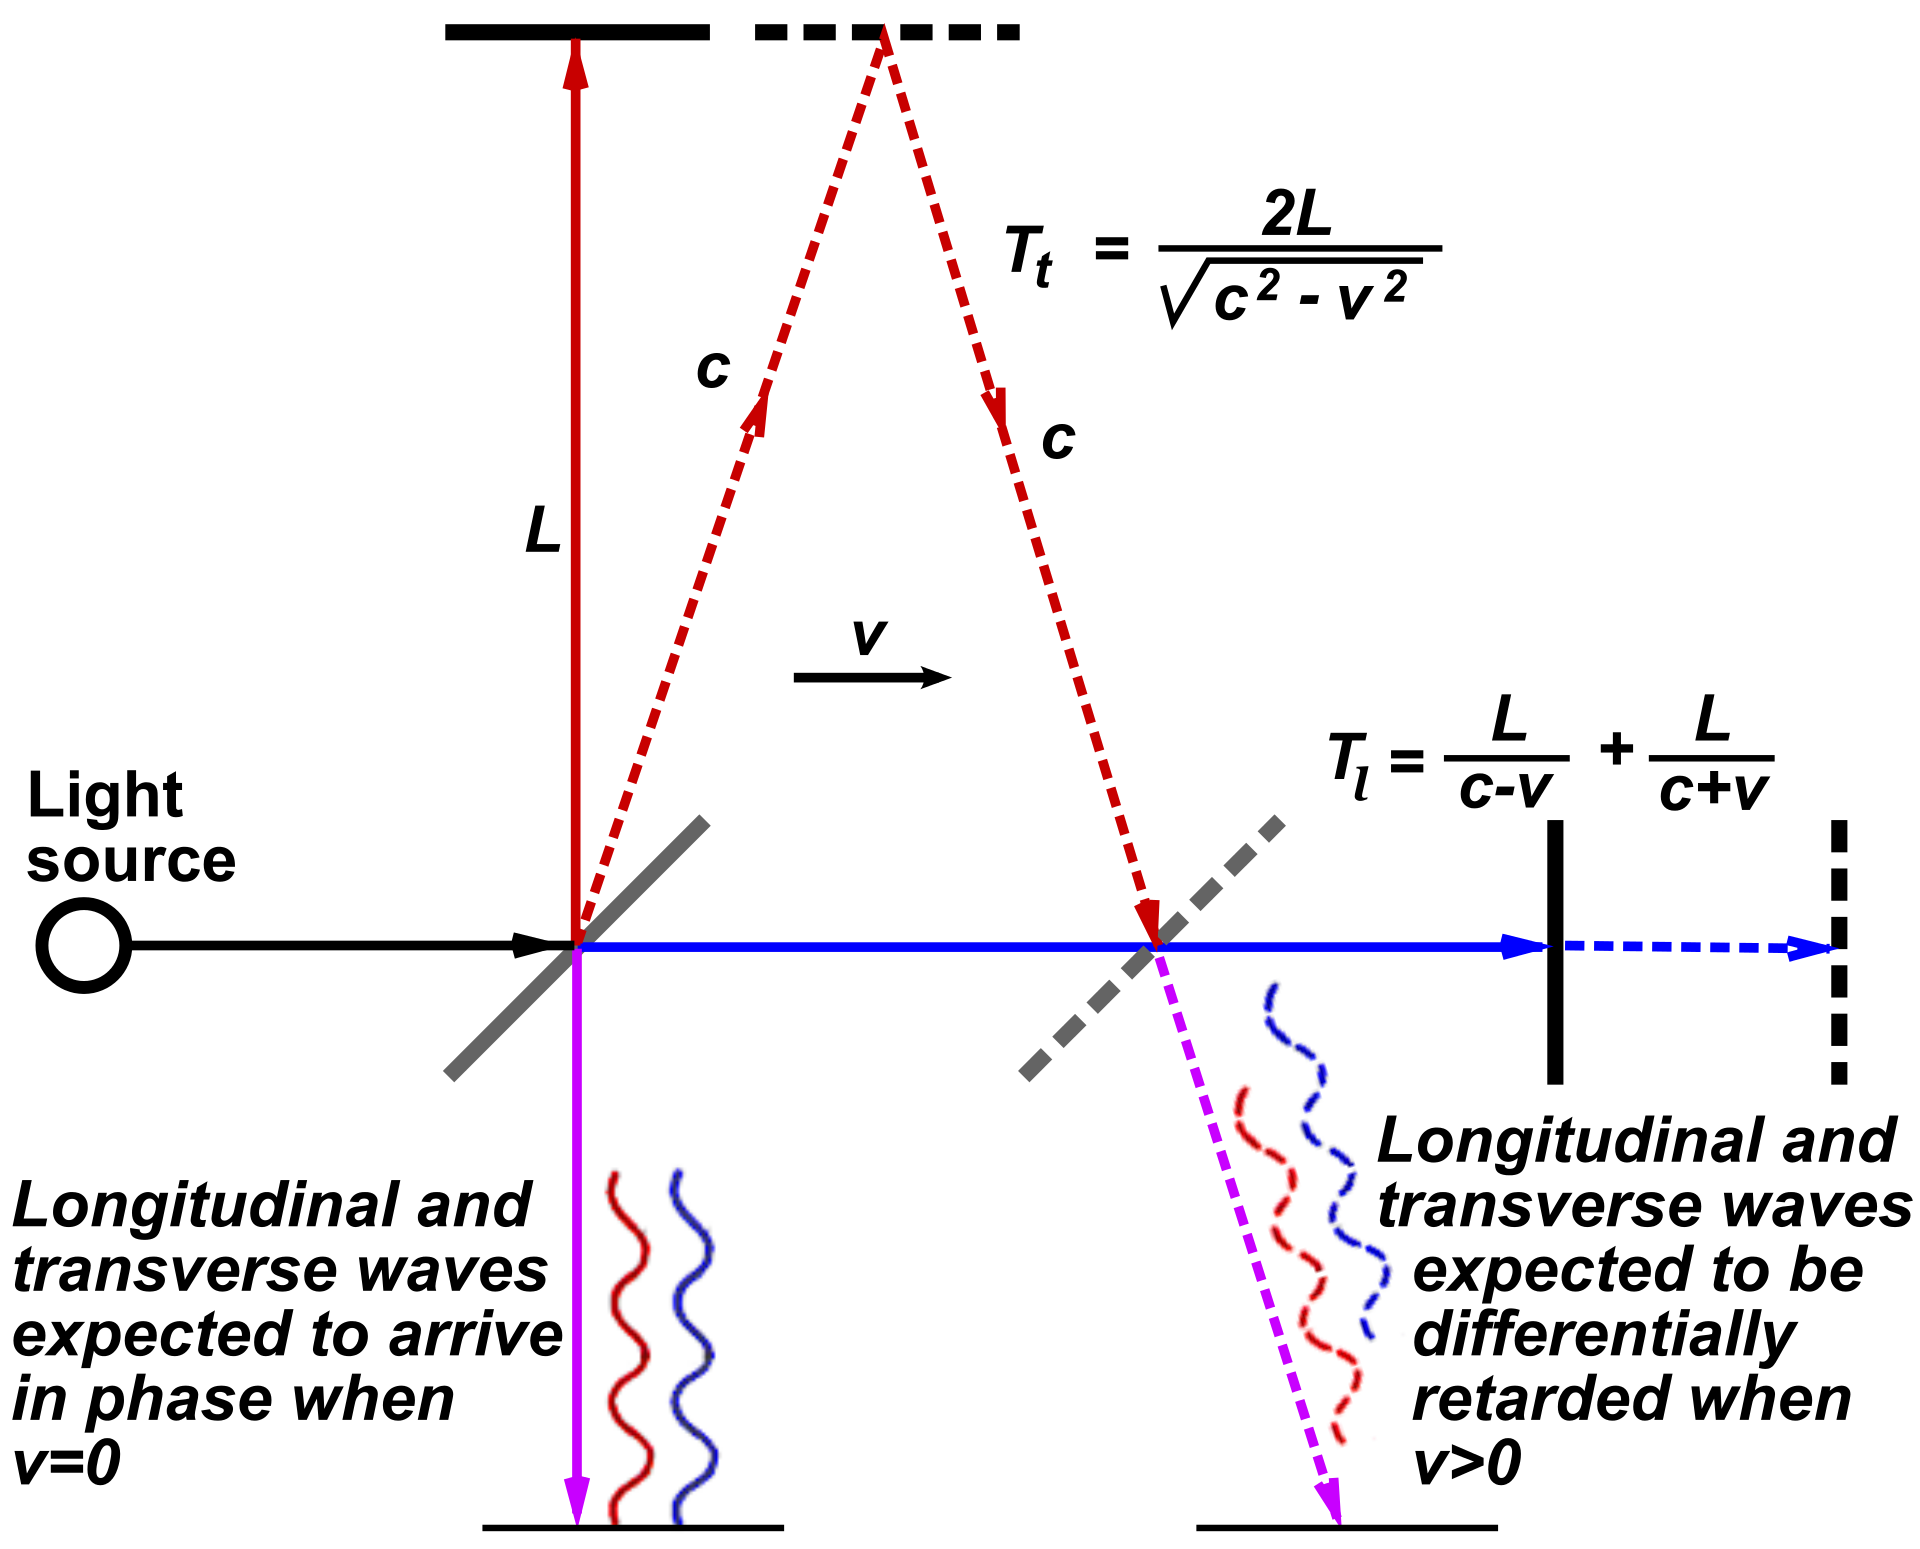
\includegraphics[width=20em,keepaspectratio]{./pictures/4.png}

          \vspace{1em}

    \item 热辐射实验-紫外灾难: 紫外波段辐射能量在当时理论下应为$\infty$,实际辐射能量为$0$

          \vspace{1em}

          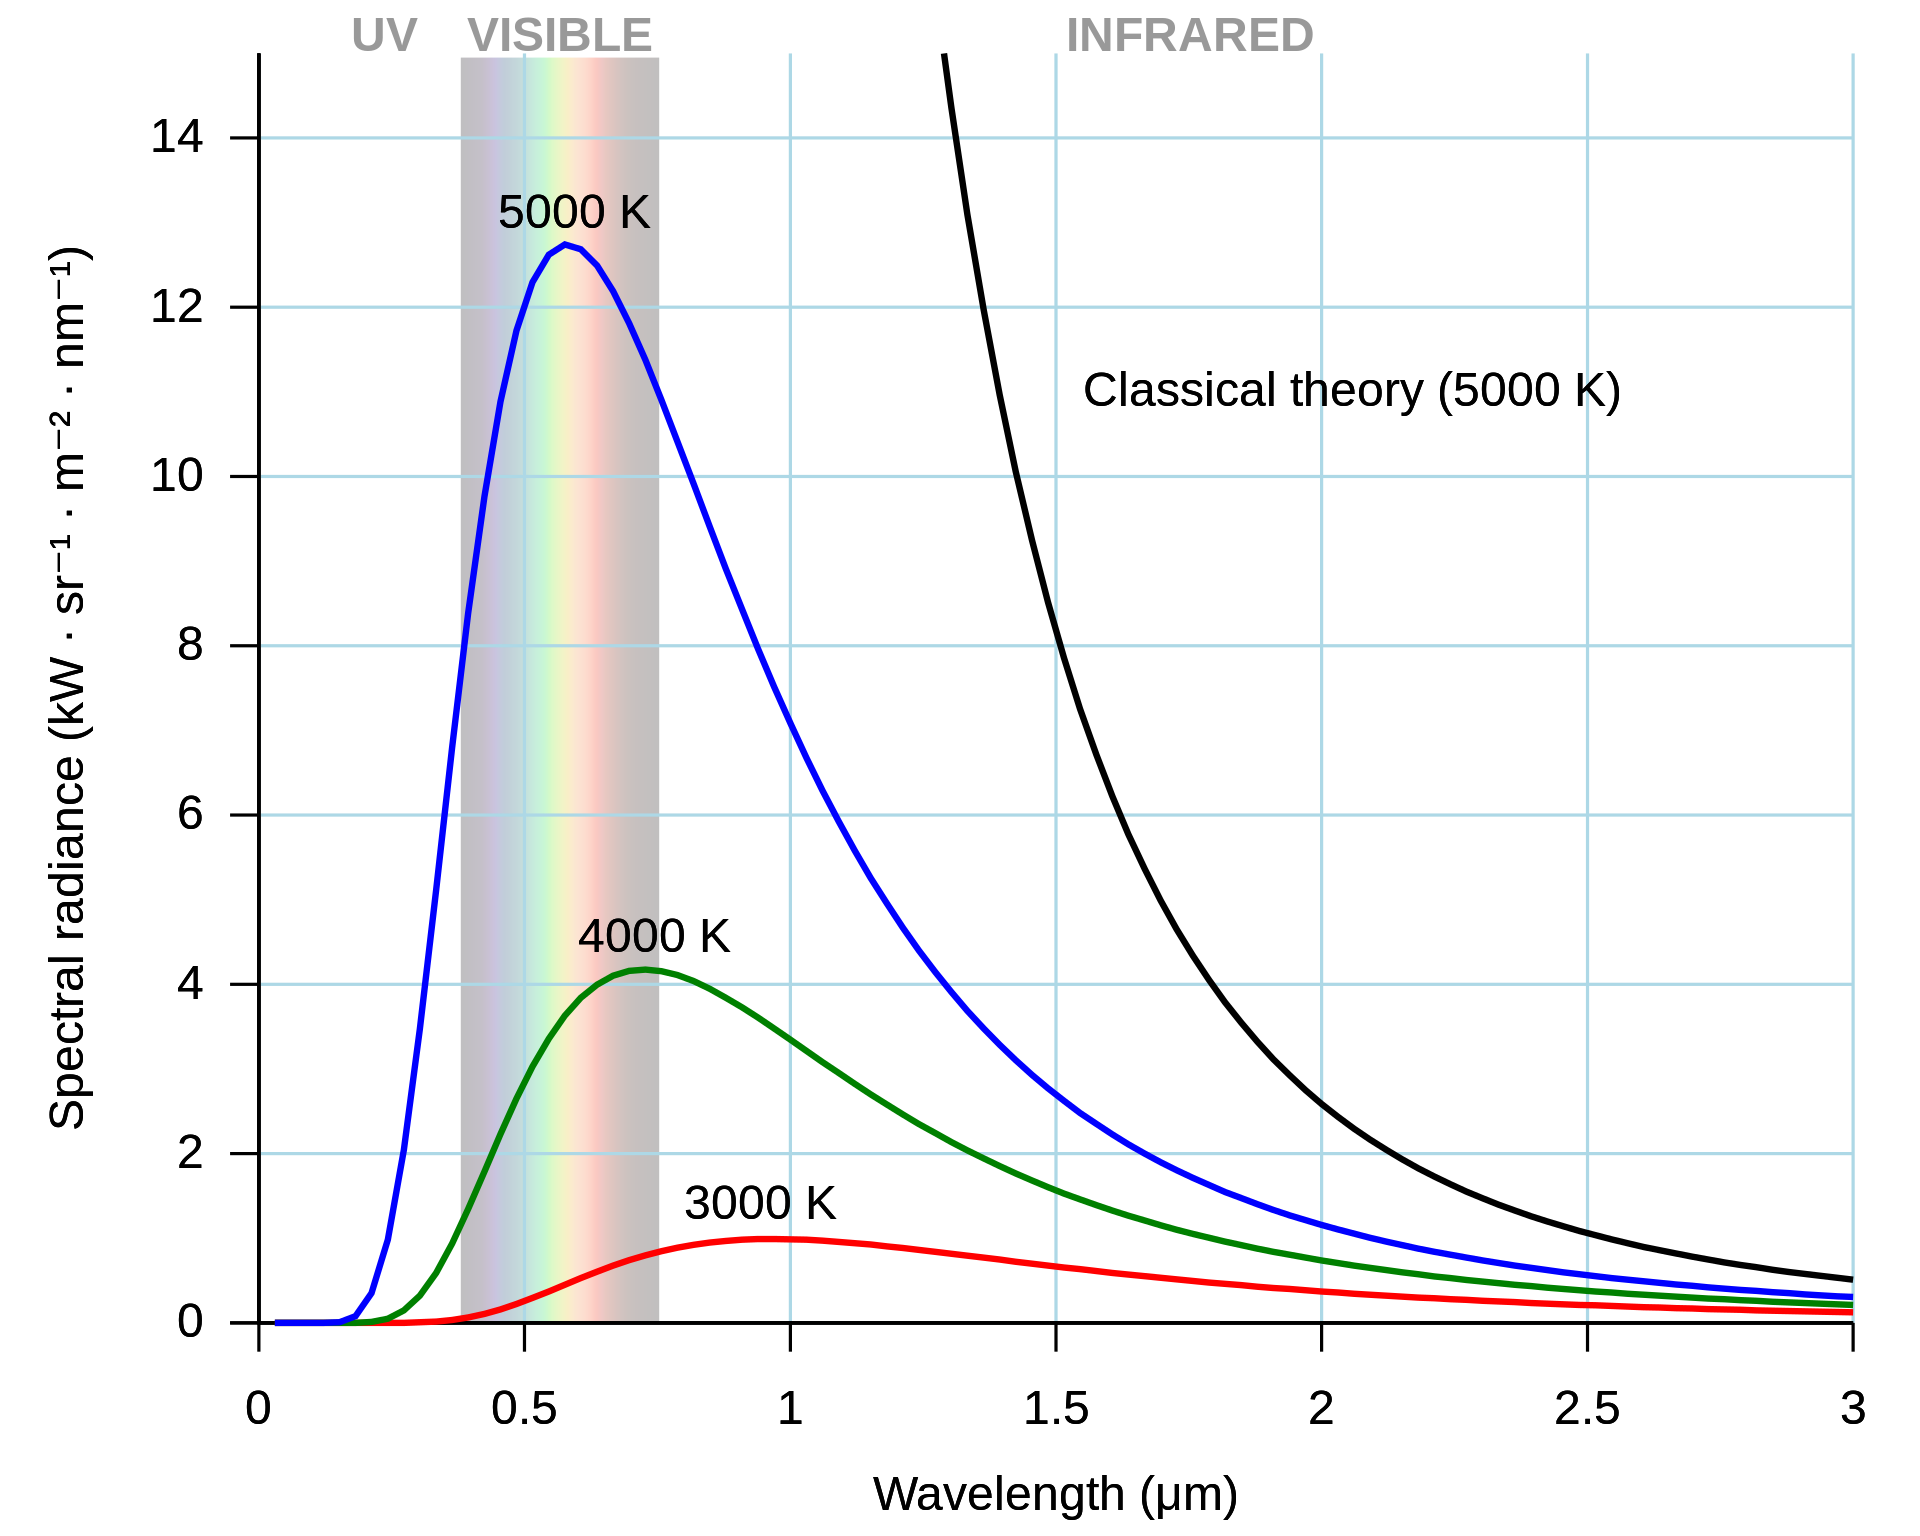
\includegraphics[width=20em,keepaspectratio]{./pictures/5.png}
          \begin{itemize}
              \item 在特定温度下,辐射的电磁波波段范围较广,强度不一
              \item 随着温度的升高,辐射出的各个波长的
          \end{itemize}
\end{itemize}

\vspace{2em}

\subsubsection{为什么要研究辐射}
\begin{itemize}
    \item 各个国家都在大炼钢铁(大炼钢时代),资本家为了提高炼钢技术请物理学家进行研究
    \item 热辐射: 任何物体都在进行热辐射(电磁波),且与\textbf{温度}(非唯一)有关
    \item 物理学家尝试测量最好炼钢温度所产生的热辐射(电磁波波谱)
\end{itemize}

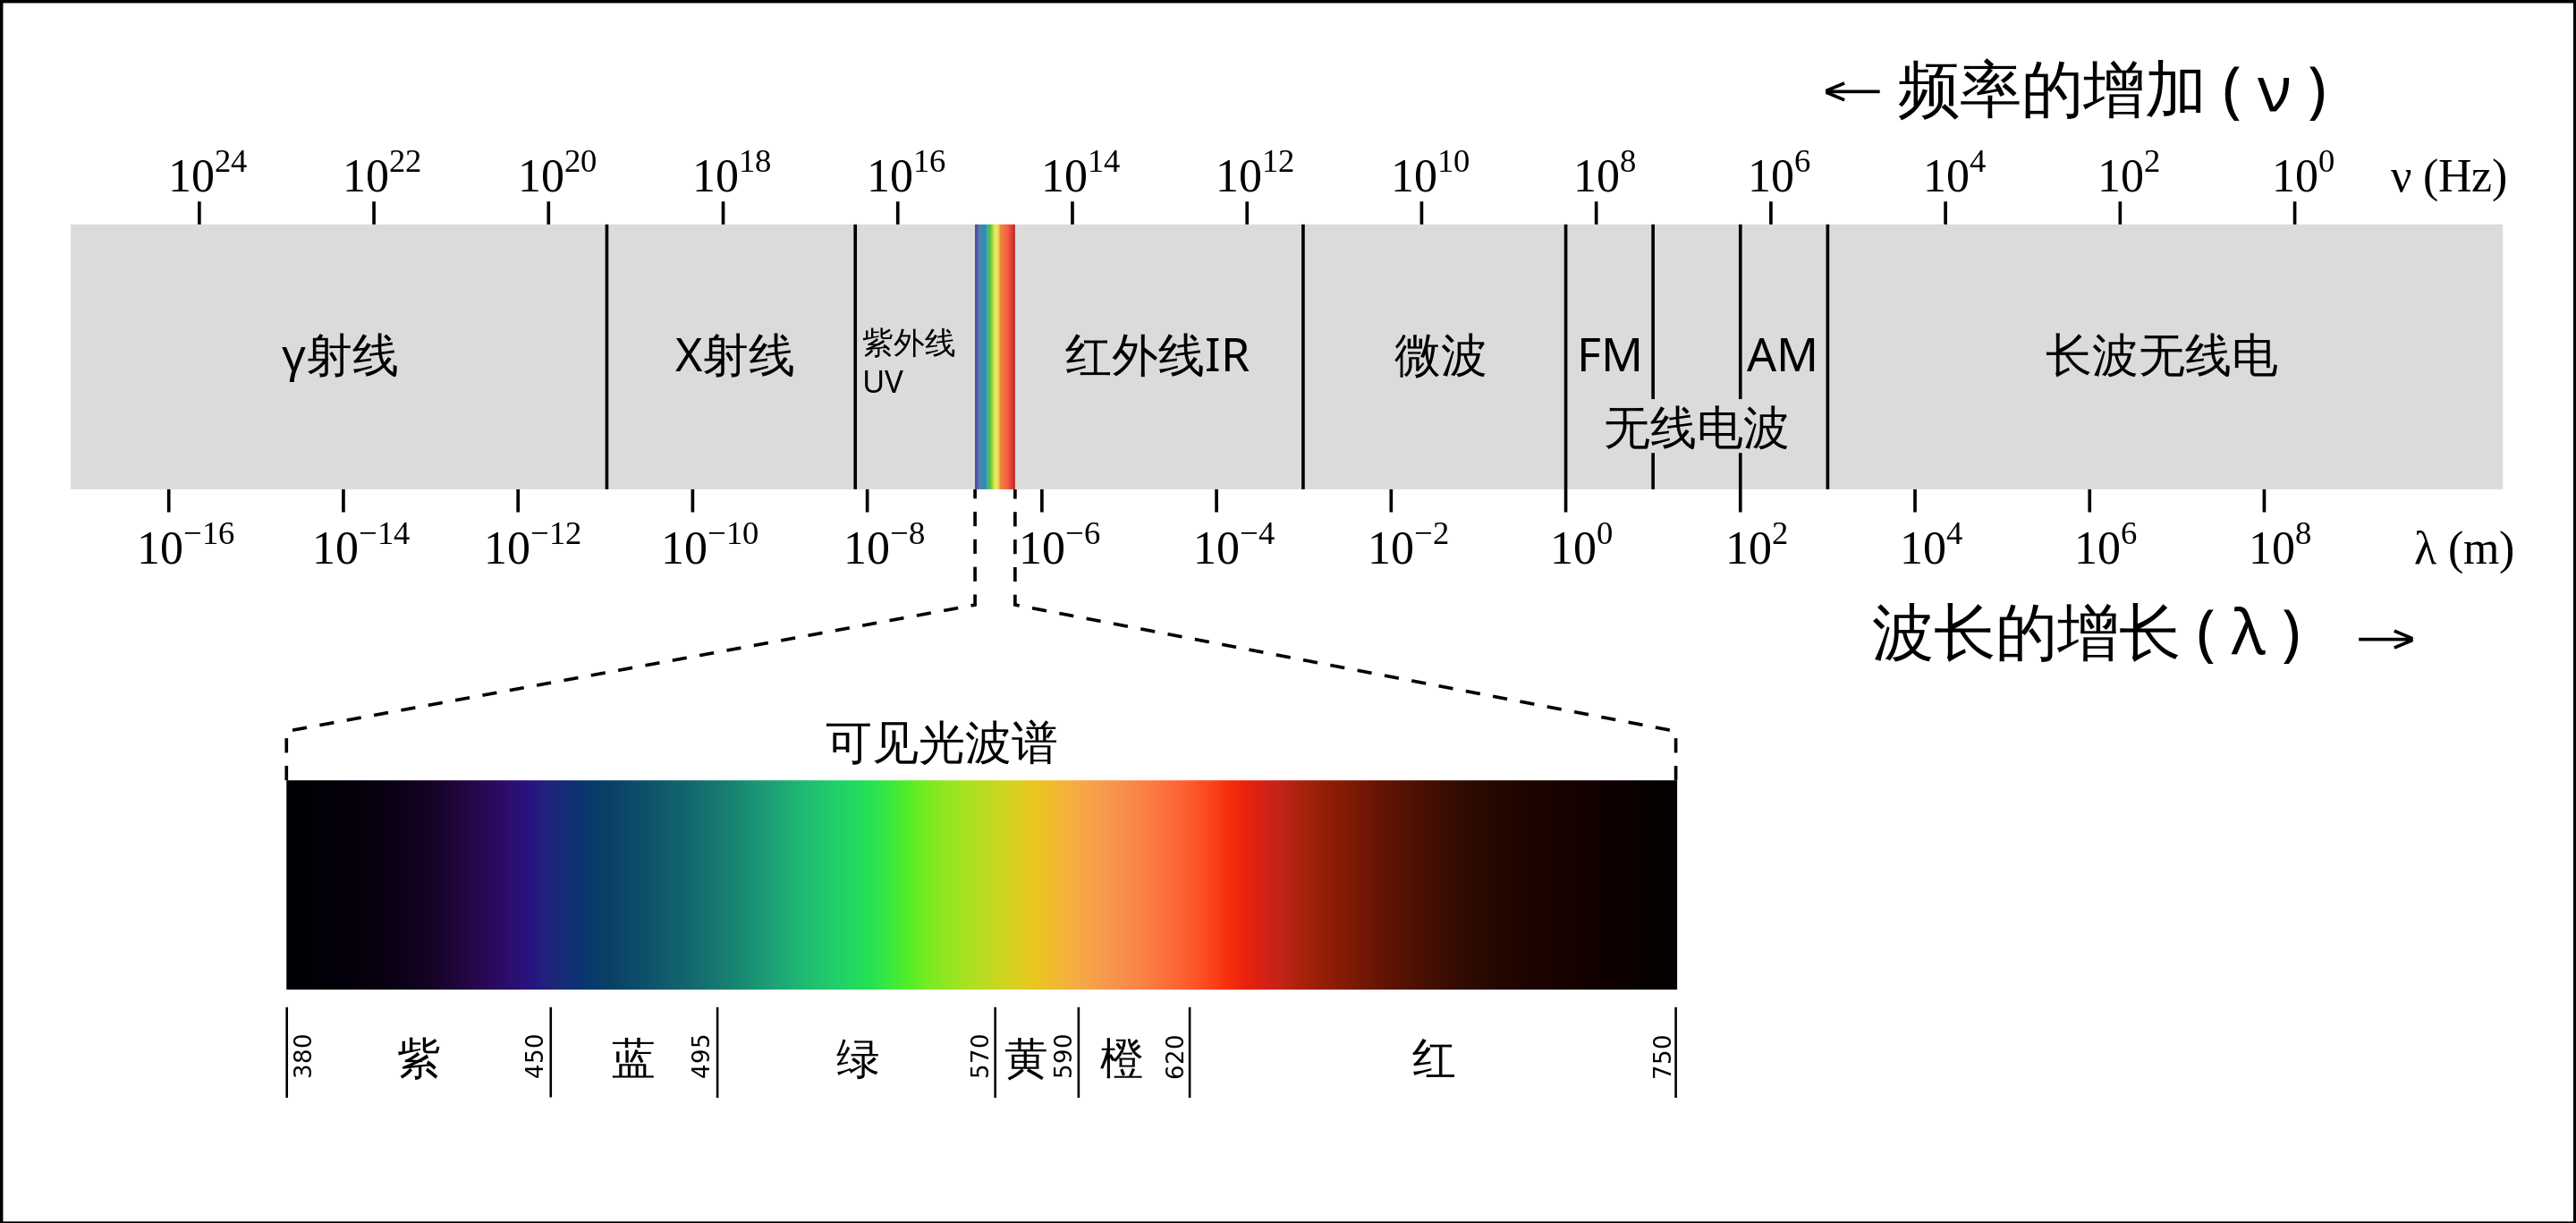
\includegraphics[width=37em,keepaspectratio]{./pictures/6.png}

\vspace{2em}

\subsubsection{黑体模型}
\begin{itemize}
    \item 理想黑体概念: 反射率与透射率为$0$,吸收率$100\%$,全靠自身发射辐射
          \begin{itemize}
              \item[] 常见近似黑体: 太阳 \, 发光灯泡 \, 钻孔箱
          \end{itemize}
\end{itemize}











\end{document}